\chapter{Introduction}

Le VDR-4 est un appareil de ventilation à haute fréquence conçu au cours des
années 1980\cite{Vienne2008} par l'inventeur américain Forest Morton Bird.  Il a été conçu en
tant qu'appareil de ventilation universel, capable de ventiler adéquatement
n'importe quel poumon humain, sain ou gravement malade, de la clientèle
néonatale à la clientèle adulte.  Son développement a été motivé par le constat
que la ventilation mécanique en pression positive conventionnelle (c'est-à-dire
basée sur un volume courant et une fréquence physiologiques) était peu adaptée
à la ventilation d'un patient présentant une pathologie pulmonaire inhomogène
(MPOC, pneumonie, brûlure d'inhalation, SDRA, etc.).

Outre le type singulier de ventilation qu'il délivre \footnote{Voir
section~\ref{sec:particularite}}, le VDR-4 se distingue aussi par son
fonctionnement entièrement pneumatique. Ceci lui confère l'avantage de
fonctionner indépendament de toute alimentation électrique. En contrepartie,
l'appareil a des capacités de monitorage très limitées, et une interface
utilisateur peu conviviale.

\section{Vocabulaire}

\begin{description}
	\item[Convection:] Déplacement d'un volume de gaz. Lors de la ventilation
	<<conventionnelle>>, les échanges gazeux entre le circuit du ventilateur et
	les bronchioles terminales se font par convection\cite{West2017}. On peut donc parler de
		ventilation \em{convective}.  
	\item [Diffusion:] Déplacement des molécules d'un gaz à l'intérieur d'un mélange gazeux. Les molécules d'un gaz diffusent en suivant leur gradient de concentration.
	\item [Hertz:] Unité de mesure de fréquence correspondant à un cycle par seconde ou soixante cycles par minute.
	\item [Iatrogène:] Causé par la thérapie.
	\item [Percussion:] Bref jet de gaz à haute vélocité.
	\item [Pression motrice:] Dans un contexte de ventilation par VDR-4, on désigne pression motrice la différence entre la pression moyenne à l'inspiration et la pression moyenne à l'expiration.
	\item [Pression partielle:] Pression exercée par les molécules d'un gaz à l'intérieur d'un mélange gazeux.
\end{description}

\section{Notions de ventilation à haute fréquence}

Ce qui caractérise la ventilation à haute fréquence est l'administration de
volumes courants inférieurs au volume de l'espace mort anatomique du patient.
Les échanges gazeux entre les alvéoles et le circuit de ventilation s'y font
selon un ensemble de mécanismes différents. À ce jour, l'influence respective
de chacun de ces mécanismes reste encore à élucider\cite{Pillow2005}.

\subsection{Oxygénation lors de la ventilation à haute fréquence}

Les facteurs influençant l'oxygénation lors de la ventilation à haute fréquence
sont, à toute fin pratique, les mêmes que pour la ventilation convective.

Dans l'absolu, l'oxygénation du sang est proportionnelle à la pression
partielle d'oxygène dans les alvéoles. Les trois principales variables
influençant cette pression partielle sont: la concentration d'oxygène dans
l'air insufflé, la pression alvéolaire moyenne, la concentration alvéolaire de
gaz carbonique.

\subsection{Relation fréquence-volume-ventilation}

Ce qui limite les volumes courants en ventilation à haute fréquence est le peu
de temps disponible pour chaque cycle respiratoire. Ce temps est d'autant plus
court que la fréquence est élevée. 
\marginpar{%
$$ {T_{cycle}}{(s)} = \frac{60}{Freq{(/m)}}$$%
}
En conséquence, une diminution de la fréquence entrainera une augmentation du
volume courant en laissant plus de temps à la pression pour s'équilibrer entre
le circuit et les alvéoles. Inversement, une augmentation de la fréquence
entrainera une diminution du volume courant.

Ainsi, en ventilation à haute fréquence, une diminution de la fréquence
favorise une plus grande élimination du $CO_2$.

Il a été démontré que la fréquence est un paramètre très important pour
l'élimination du $CO_2$ en ventilation à haute fréquence\cite{Pillow2005}.

\section{Particularité du VDR-4}
\label{sec:particularite}
Le VDR-4 se distingue des autres appareils de ventilation à haute
fréquence par l'alternance (à basse fréquence) entre deux (voire même
trois) amplitudes de percussion. Il en résulte une alternance entre
deux pressions moyennes. Les échanges gazeux lors de ce type de
ventilation seront, par conséquent, à la fois le résultat du
déplacement de grands volumes d'air (convection) et de l'ensemle de
mécanismes d'échanges gazeux propres à la ventilation à haute
fréquence.

\begin{SCfigure}
	\begin{wide}
	\tikzsetnextfilename{fig-lfhf}

\pgfplotsset{
	lfhf/.style={
		height = 0.42 \textheight,
		enlarge y limits = {value=0.9, upper},
		enlarge x limits = false
		}
}

\tikzset{
	zoomline/.style={
		opacity=1,
		dotted
	},
	plage/.style={
		<->
	}
}

\def\zstart{7.2}
\def\zend{7.8}
\newcommand{\istart}{2}
\newcommand{\tic}{2}
\newcommand{\pstart}{7.365}
\newcommand{\tip}{0.059}

\begin{tikzpicture}
	\begin{groupplot}[
			group style={
				group size=1 by 2,
				y descriptions at=edge left,
				xlabels at=edge bottom
				},
				ylabel=Pression (hPa),
				xlabel=Temps (s),
				max space between ticks=40,
			]
		\nextgroupplot[lfhf, width=\textwidth, height=5cm]

		\addplot []table[x=time, y=Pao] {dat/simvent1.dat};


		\coordinate (PSO) at (axis cs:\zstart,0);
		\coordinate (PSE) at (axis cs:\zend,0);
		\coordinate (PNO) at (axis cs:\zstart,\pgfkeysvalueof{/pgfplots/ymax});
		\coordinate (PNE) at (axis cs:\zend,\pgfkeysvalueof{/pgfplots/ymax});

		\draw [plage](axis cs:\istart,45) -- (axis cs:\istart + \tic, 45) node[midway, above] {Inspi.};
		\draw [plage](axis cs:\istart + \tic,45) -- (axis cs:\istart + 2*\tic, 45) node[midway, above] {Expi.};

		\draw [dashed] 
		(axis cs: \istart,\pgfkeysvalueof{/pgfplots/ymax}) -- (axis cs:\istart,0)
	 	(axis cs: \istart + \tic,\pgfkeysvalueof{/pgfplots/ymax}) -- (axis cs:\istart + \tic,0)
		(axis cs: \istart + 2 *\tic,\pgfkeysvalueof{/pgfplots/ymax}) -- (axis cs:\istart + 2*\tic,0);

		%\fill [opacity=0.15] (PSO) rectangle (PNE);
		\draw [zoomline] (PSO) rectangle (PNE);


		\nextgroupplot[lfhf,
				max space between ticks=80,
				width=0.75\textwidth,
				height=5cm,
				axis background/.style={fill=gray!15, opacity=0.8},
				]
		\addplot [restrict x to domain=\zstart:\zend]table[x=time, y=Pao] {dat/simvent1.dat};

		\coordinate (ZNO) at (axis cs:\zstart,\pgfkeysvalueof{/pgfplots/ymax});
		\coordinate (ZNE) at (axis cs:\zend,\pgfkeysvalueof{/pgfplots/ymax});
		\coordinate (ZSO) at (axis cs:\zstart,\pgfkeysvalueof{/pgfplots/ymin});
		\coordinate (ZSE) at (axis cs:\zend,\pgfkeysvalueof{/pgfplots/ymin});


		\draw [dashed] 
		(axis cs: \pstart,\pgfkeysvalueof{/pgfplots/ymax}) -- (axis cs:\pstart,0)
		(axis cs: \pstart + \tip,\pgfkeysvalueof{/pgfplots/ymax}) -- (axis cs:\pstart + \tip,0)
		(axis cs: \pstart + 2 *\tip,\pgfkeysvalueof{/pgfplots/ymax}) -- (axis cs:\pstart + 2*\tip,0);
		\draw [plage] (axis cs:\pstart,45) -- (axis cs:\pstart + \tip, 45) node[midway, above] {Ins.};
		\draw [plage](axis cs:\pstart + \tip,45) -- (axis cs:\pstart + 2*\tip, 45) node[midway, above] {Exp.};

	\end{groupplot}

	\begin{scope}[on background layer]
		%\fill [opacity=0.03](ZNO) -- (PNO) -- (PNE) -- (ZNE) -- (ZNO);
		%\fill [opacity=0.03](ZSO) -- (PSO) -- (PNO) -- (PNE) -- (PSE) -- (ZSE) -- (ZSO);
		\fill [opacity=0.1](PSO) -- (PNO) -- (PNE) -- (PSE);
		%\fill [opacity=0.05](ZNE) -- (PNE) -- (PSE) -- (ZSE) -- (ZNE);
		\draw [zoomline](ZNO) -- (PNO) (PNE) -- (ZNE) ;
		\draw [zoomline](ZSO) -- (PSO) (PSE) -- (ZSE) ;
	\end{scope}

\end{tikzpicture}

	\caption[Tracé pression - temps typique.]{L'alternance entre deux
	amplitudes de percussions donne une apparence typique au tracé de la
	pression à l'ouverture des voies aériennes lors de la ventilation
	avec un VDR-4. Les phases inspiratoires et expiratoires à basse
	fréquence (courbe du haut) sont composées d'une succession
	d'inspirations et d'expirations à haute fréquence (courbe du bas).}
	\end{wide}
\end{SCfigure}

\section{Composantes du système}

\subsection{Module de contrôle}

\marginnote{%
	\begin{minipage}{0.49\textwidth}
	\centering
		\vspace{.25cm}
	\begin{tikzpicture}
		\pic [name=C] {cartouche};
		\pic {obturateur-bas};

		\draw [double distance=5.3mm,]
		(CO) -- ++(2,0) (CO) ++ (1,0) |- (CS)
		node [pos=0.25] {$\downarrow$}
		node [pos=0.75] {$\leftarrow$}
		;

		\draw (CI) node {$\downarrow$};
		\draw (CO) node {$\rightarrow$};

	\end{tikzpicture}
	A - Cartouche ouverte

\end{minipage}
\begin{minipage}{0.49\textwidth}
	\centering
		\vspace{.25cm}
	\begin{tikzpicture}

		\pic [name=C] {cartouche};
		\pic {obturateur-haut};

		\draw [double distance=5.3mm,]
		(CO) -- ++(2,0) (CO) ++ (1,0) |- (CS) 
		;

		\draw (CI) node {$\downarrow$};

	\end{tikzpicture}
	B - Cartouche fermée

\end{minipage}

	\captionof{figure}[Fonctionnement d'une cartouche pneumatique.]{Fonctionnement d'une cartouche pneumatique. À mesure que la pression
	augmente derrière le diaphragme, celui-ci se déforme, emmenant  le piston à
	obstruer l'arrivée de gaz.} 
	}[-8cm]

Le module de contrôle est la composante qui permet de régler les
paramètres de la ventilation délivrée par le VDR-4.  À partir de son
alimentation en gaz à haute pression (air et oxygène), le module de
contrôle produit:

\begin{itemize}
	\item Un débit intermittent alimentant le phasitron (connecteur et
		tubulure blanche),
	\item Un débit continu (+/- 20 l/min) alimentant
		le nébuliseur ou tout autre système d'humidification (si activé)
		(connecteur et tubulure jaune),
	\item Un débit auxiliaire (+/- 10 l/min) ajouté à la sortie du
		nébuliseur (dans le circuit classique) (connecteur et tubulure
		verte).
\end{itemize}

Il est aussi doté d'un port de monitorage (connecteur et tubulure
rouge).  Un multimètre numérique -- situé sur le dessus de l'appareil
-- affiche les pressions moyennes (inspiratoire, expiratoire et
globale) et les fréquences (percussion et convection).  Finalement, le
module de contrôle comprend aussi une alarme de déconnexion alimentée
par une pile (située sur le côté droit de l'appareil).

Le fonctionnement du module de contrôle est exclusivement pneumatique,
à l'exception du multimètre et de l'alarme de déconnexion.  Chaque
bouton actionné par l'utilisateur est une valve contrôlant une
cartouche pneumatique. 

Le circuit logique du module de contrôle est constitué d'un agencement
d'une dizaine de cartouches pneumatiques.  Cette conception a pour
résultat que plusieurs paramètres réglables s'interinfluencent.  Par
exemple, une augmentation de l'amplitude des percussions à
l'inspiration (bouton DEBIT PULSE) entrainera aussi une augmentation
de l'amplitude des percussions à l'expiration.

\begin{figure}[t]
	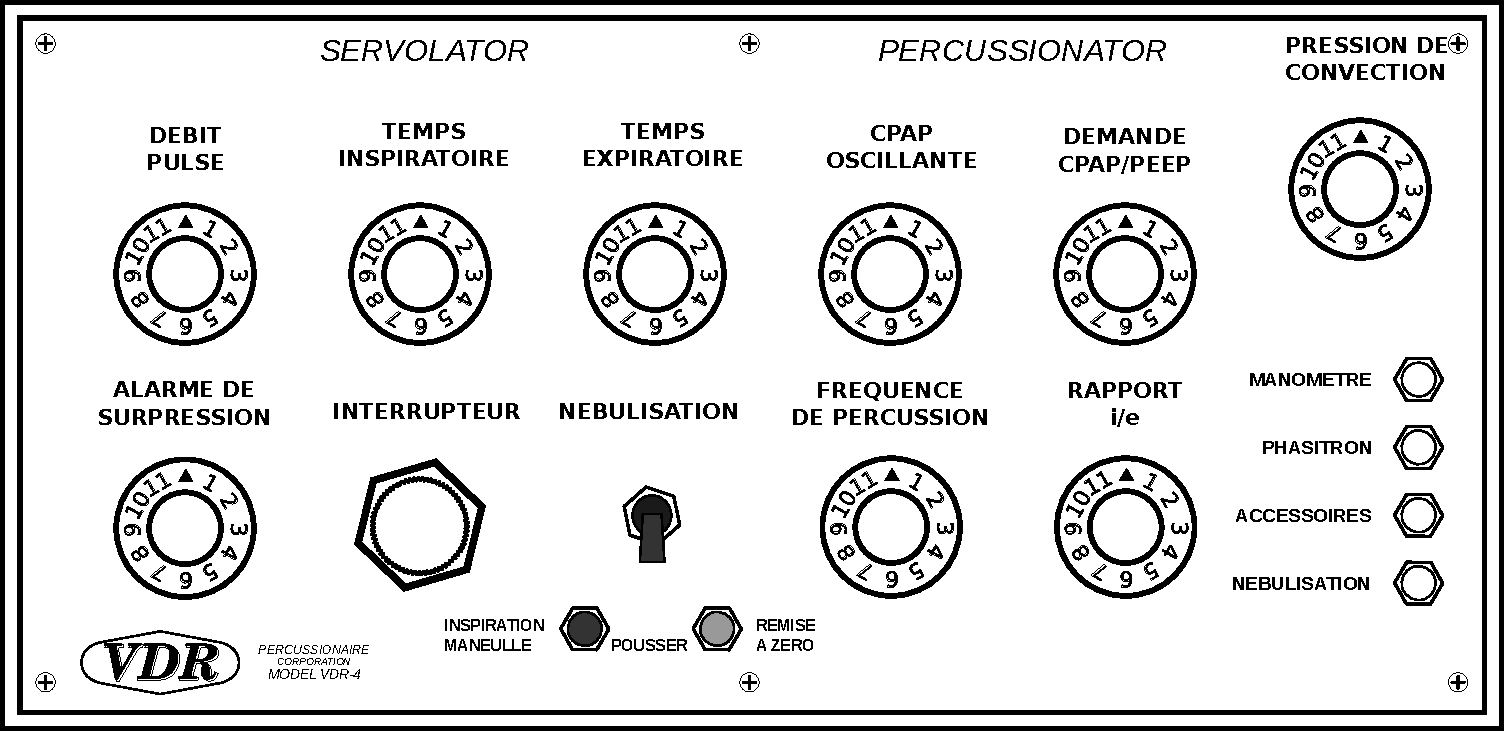
\includegraphics[width=\textwidth]{img/Module_de_controle}
	\caption{Panneau avant du module de contrôle.}
\end{figure}

\subsection{Phasitron}
\index{phasitron}

Le phasitron est la composante du circuit de ventilation raccordée
directement à l'interface patient (tube endotrachéal, canule de
trachéotomie, etc.). Il remplit les deux fonctions suivantes: 

\begin{itemize} 
	\item Amplification du jet de gaz (percussion) en provenance du
		module de contrôle,
	\item Valve expiratoire.
\end{itemize}

\marginnote{%
	\def\pScale{0.5}
\centering
\begin{minipage}{.45\textwidth}
	\centering
	\tikzsetnextfilename{fig-phasitron_inspi}
	\begin{tikzpicture}[
			scale=\pScale,
			every node/.style={transform shape}
			]

			\pic [name=P, draw=black!50, fill=gray!10] {phasitron-coupe};
			\pic {venturi-avance};
			\path (P-S) -- (P-Pt) 
			node [pos=0.32] (J) {}
			coordinate [pos=0.15] (D)
			;


			\draw [line width=.2mm, ->] (P-S) ++(3mm,0) to (D);
			\draw [
				line width=.2mm,
				->, 
				shorten <=1mm,
				] (D) to (J);

				\draw [
					line width=.5mm, 
					->, 
					out=90, 
					in=-45,
					shorten >=1mm
					] (P-A) ++ (0, -3mm)  to (J);

					\draw [line width=1mm, ->] (J)  to (P-Pt);

	\end{tikzpicture}

	A - Inspiration
\end{minipage}\hfill
\begin{minipage}{0.45\textwidth}
	\centering

	\tikzsetnextfilename{fig-phasitron_expi}
		\begin{tikzpicture}[
				scale=\pScale,
				every node/.style={transform shape}
				]

				\pic [name=P, draw=black!50, fill=gray!10] {phasitron-coupe};
				\pic {venturi-recule};

				\draw [
					line width=1mm, 
					->, 
					out=0, 
					in=90, 
					looseness=1.8,
					] ([yshift=-4mm]P-Pt) to (P-E);

		\end{tikzpicture}

		B - Expiration
\end{minipage}

	\captionof{figure}[Fonctionnement du phasitron.]{Fonctionnement du phasitron.
	Le débit en provenance du module de contrôle déforme le diaphragme
	et déplace le tube de venturi vers l'avant lors de l'inspiration,
	obstruant ainsi l'orifice expiratoire. À l'expiration, le diaphragme
	reprend sa forme initiale et ramène le tube de venturi vers
	l'arrière, libérant ainsi l'orifice expiratoire.} 
	\label{fig:phasitron-coupe}
	}[-8cm]
L'amplification du jet de gaz se fait par un appel d'air (principe de
venturi).  Le ratio \emph{air aspiré: air injecté} du tube de venturi
diminue au fur et à mesure que la pression augmente à la sortie de
celui-ci. Conçu en tant que mécanisme de protection pulmonaire, cette
caractéristique tend à diminuer l'amplitude des variations de
pressions de ventilation lors de changements de mécanique pulmonaire.

Lorsqu'un débit d'air est injecté dans le tube de venturi, il se
déplace vers l'avant du phasitron, obstruant ainsi l'orifice
expiratoire (voir Figure \ref{fig:phasitron-coupe}). Lorsque le tube
de venturi ne reçoit plus de débit, il retourne à sa position de repos
(à l'arrière du phasitron), libérant ainsi l'orifice expiratoire.

L'absence de circuit respiratoire entre le phasitron et l'interface
patient ainsi que l'utilisation de tubulures peu compliantes entre le
phasitron et le module de contrôle évitent l'atténuation des
percussions dans le volume compressible du circuit.

\begin{figure}
	\begin{tikzpicture}[
		every node/.style={
			align=center
		}
]
\pic [name=Phasitron, scale=0.5] {phasitron};
	\node [left=2mm] at (Phasitron-Pt) {Patient $\leftrightarrow$};
	\node [below=2mm] at (Phasitron-E) {$\downarrow$\\Expiration};
	\node [below=2mm, align=center] at (Phasitron-A) {$\uparrow$\\Appel d'air};
	\node [right=2mm] at (Phasitron-S) {$\leftarrow$ Pressurisation};
	\node [below=2mm, anchor=north east] at (Phasitron-M) {Monitorage};
\end{tikzpicture}

	\caption{Le phasitron.}
\end{figure}

\subsection{Système d'humidification}

Le système d'humidification de base du VDR-4 est un nébuliseur pneumatique.
Celui-ci est utilisé pour humidifier les gaz qui sont aspirés par le tube de
venturi du phasitron. Le circuit d'humidification est conçu de façon à:

\begin{itemize}
	\item S'assurer qu'un débit suffisant est disponible à l'orifice d'appel d'air du phasitron,
	\item Évacuer le débit excédentaire,
	\item Permettre au patient de respirer facilement l'air ambiant en cas de défaillance de l'appareil.
\end{itemize}

Plusieurs institutions utilisant le VDR-4 jugent ce système 
d'humidification insuffisant et le combine ou le remplace par un 
(ou même deux) humidificateur chauffant (voir Figure \ref{fig:circ}).

\begin{figure}
	\begin{wide}
	\tikzsetnextfilename{fig-circuit}
\begin{tikzpicture}[
	scale=0.32,
	very thin,
]

\begin{scope}[every node/.style={ transform shape }]
	\pic [name=F] at(0,0) {fp};
	\pic [name=N] at(15,10) {neb};
	\pic [yscale=1.22, xscale=-1.22, name=P] at (25, 35) {phasitron};
	\pic [scale=1.8, name=VDR] at (-20,40) {vdr};
	\pic [name=M] at(N-CR) {manifold};
	\pic  at (M-BC) {bag};
\end{scope}

%%%%%%%%%%%%%%%%%%%%%%%%%%%%%%%%%%%%%%%%%%%%%%%%%%
% Hight presure  circuit
%%%%%%%%%%%%%%%%%%%%%%%%%%%%%%%%%%%%%%%%%%%%%%%%%%

\begin{scope}[every path/.style={double distance=0.8mm}]
	\draw (VDR-C1)  -| (P-M);
	\draw (VDR-C2) -- ++(8,0) |- (P-S);
	\draw (VDR-C4) -- ++(6, 0) -- ++(0, -30) -| (N-CN);
\end{scope}

\begin{scope}[every node/.style={transform shape}]
	\pic [yshift=11mm, xscale=-1] (fsa) at (P-A) {failsafeValve};
	\pic [yshift=11mm] (fse) at (P-E) {failsafeValve};
\end{scope}

%%%%%%%%%%%%%%%%%%%%%%%%%%%%%%%%%%%%%%%%%%%%%%%%%%
% Humidification circuit
%%%%%%%%%%%%%%%%%%%%%%%%%%%%%%%%%%%%%%%%%%%%%%%%%%

\begin{scope}[
	every path/.style={
		double distance=7mm,
		looseness=2,
		shorten <=-1mm,
		shorten >=-1mm
	}
]

% From the exalation to the manifold
\draw (fse-CB) to [out=-90, in=0, sloped, sloped, near start]  node {$\rightarrow$} (M-RC);

% From the nebuliser to the FishePaykel
\draw [double=black!13](N-CL) to [out=180, in=90, sloped, near start]  node {$\leftarrow$} (F-CR);

% From the FisherPaykel to the phasitron
\draw [double=black!13](F-CL) to [out=90, in=270, sloped] node {$\rightarrow$} (fsa-CB);

\end{scope}

% valves direction
\node foreach \pos in {a, e} [xscale=-1, font=\tiny] at(fs\pos-V) {$\mapsto$};

\end{tikzpicture}

	\caption{Intégration d'un humidificateur chauffant au circuit du VDR-4.}
	\label{fig:circ}
	\end{wide}
\end{figure}

\begin{figure}
	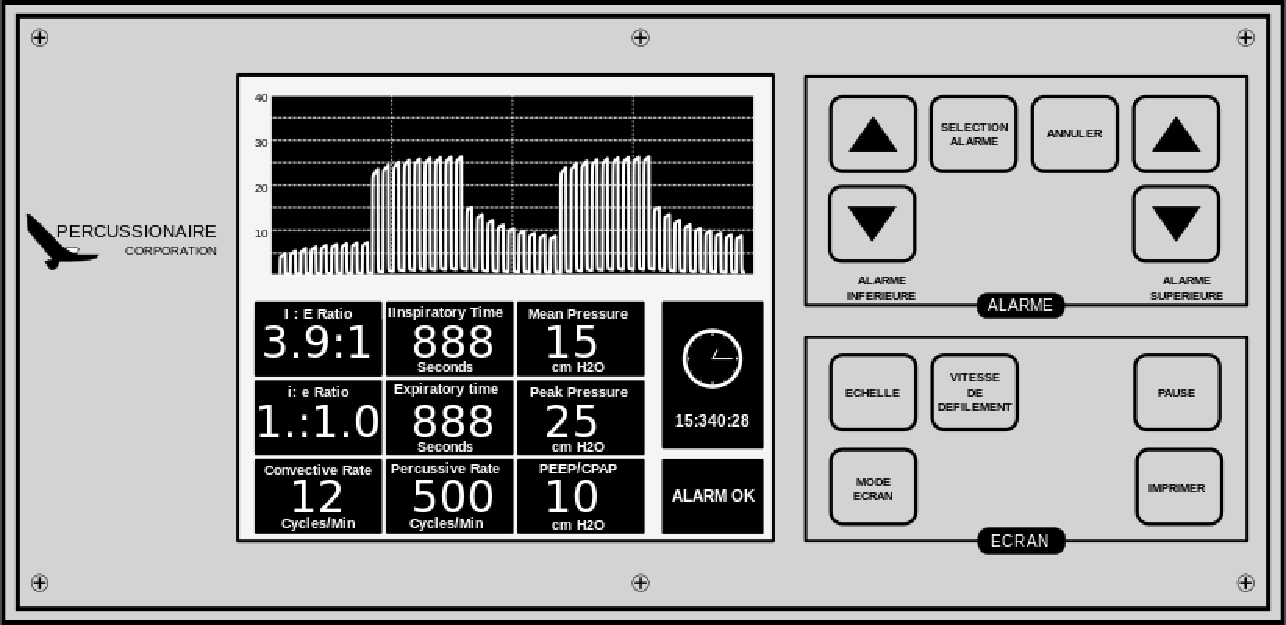
\includegraphics[width=\textwidth]{img/Monitron}
	\caption{Panneau avant du monitron.}
\end{figure}
\subsection{Module de monitorage (Monitron)}

Le Monitron est un moniteur électronique complètement indépendant du
module de contrôle. Il vise à étendre les capacités de monitorage
limitées de celui-ci.

Le signal de pression est transmis du module de contrôle au Monitron
au moyen d'une tubulure se trouvant dans l'espace entre les deux
appareils.

\subsubsection{Données monitorées}

Les données numériques fournies par le Monitron sont les suivantes:

\begin{itemize}
\item Pression de crête inspiratoire,
\item Pression de crête expiratoire,
\item Pression moyenne,
\item Temps inspiratoire (convection),
\item Temps expiratoire (convection),
\item Fréquence (convection),
\item Ratio I:E (convection),
\item Fréquence (percussion),
\item Ratio i:e (percussion),
\item Heure.
\end{itemize}

\subsubsection{Alarmes}

Une alarme de basse pression et une alarme de haute pression peuvent être ajustées.

L'alarme de haute pression se déclenche dès que la pression lue est supérieure
au seuil d'alarme réglé.

L'alarme de pression basse se déclenche lorsque la pression lue est inférieure
au seuil d'alarme réglé pour une durée supérieure à 30 secondes.

La touche SET ajuste automatiquement l'alarme basse à 2 \cmh et l'alarme haute
à 10 \cmh\ au-dessus de la pression de crête inspiratoire.

